\section{Methodology}
\subsection{Overview}
This project consists of three main units: a discharge flow control unit, a discharge collection  unit, and a software and control unit. 
\subsection{Discharge flow control unit}
This unit consist of two main sub units:
\begin{enumerate}
    \item Flow control sub-unit\\
    This unit is solely responsible for controlling the flow from the discharge pipe in steps.
    \item Flow diversion sub-unit\\
    This unit is used to divert the flow from the main pipe either to the discharge collection tank during discharge collection or to the main reservoir.
\end{enumerate}
\par
\subsubsection{Flow control  sub-unit}
The unit serves to open the main discharge pipe in steps. The current state-of-art of the Synthetic Hydro Experimental machine is as shown in figure \ref{fig:current_discharge_control_unit}. 
\begin{figure}[H]
    \centering
    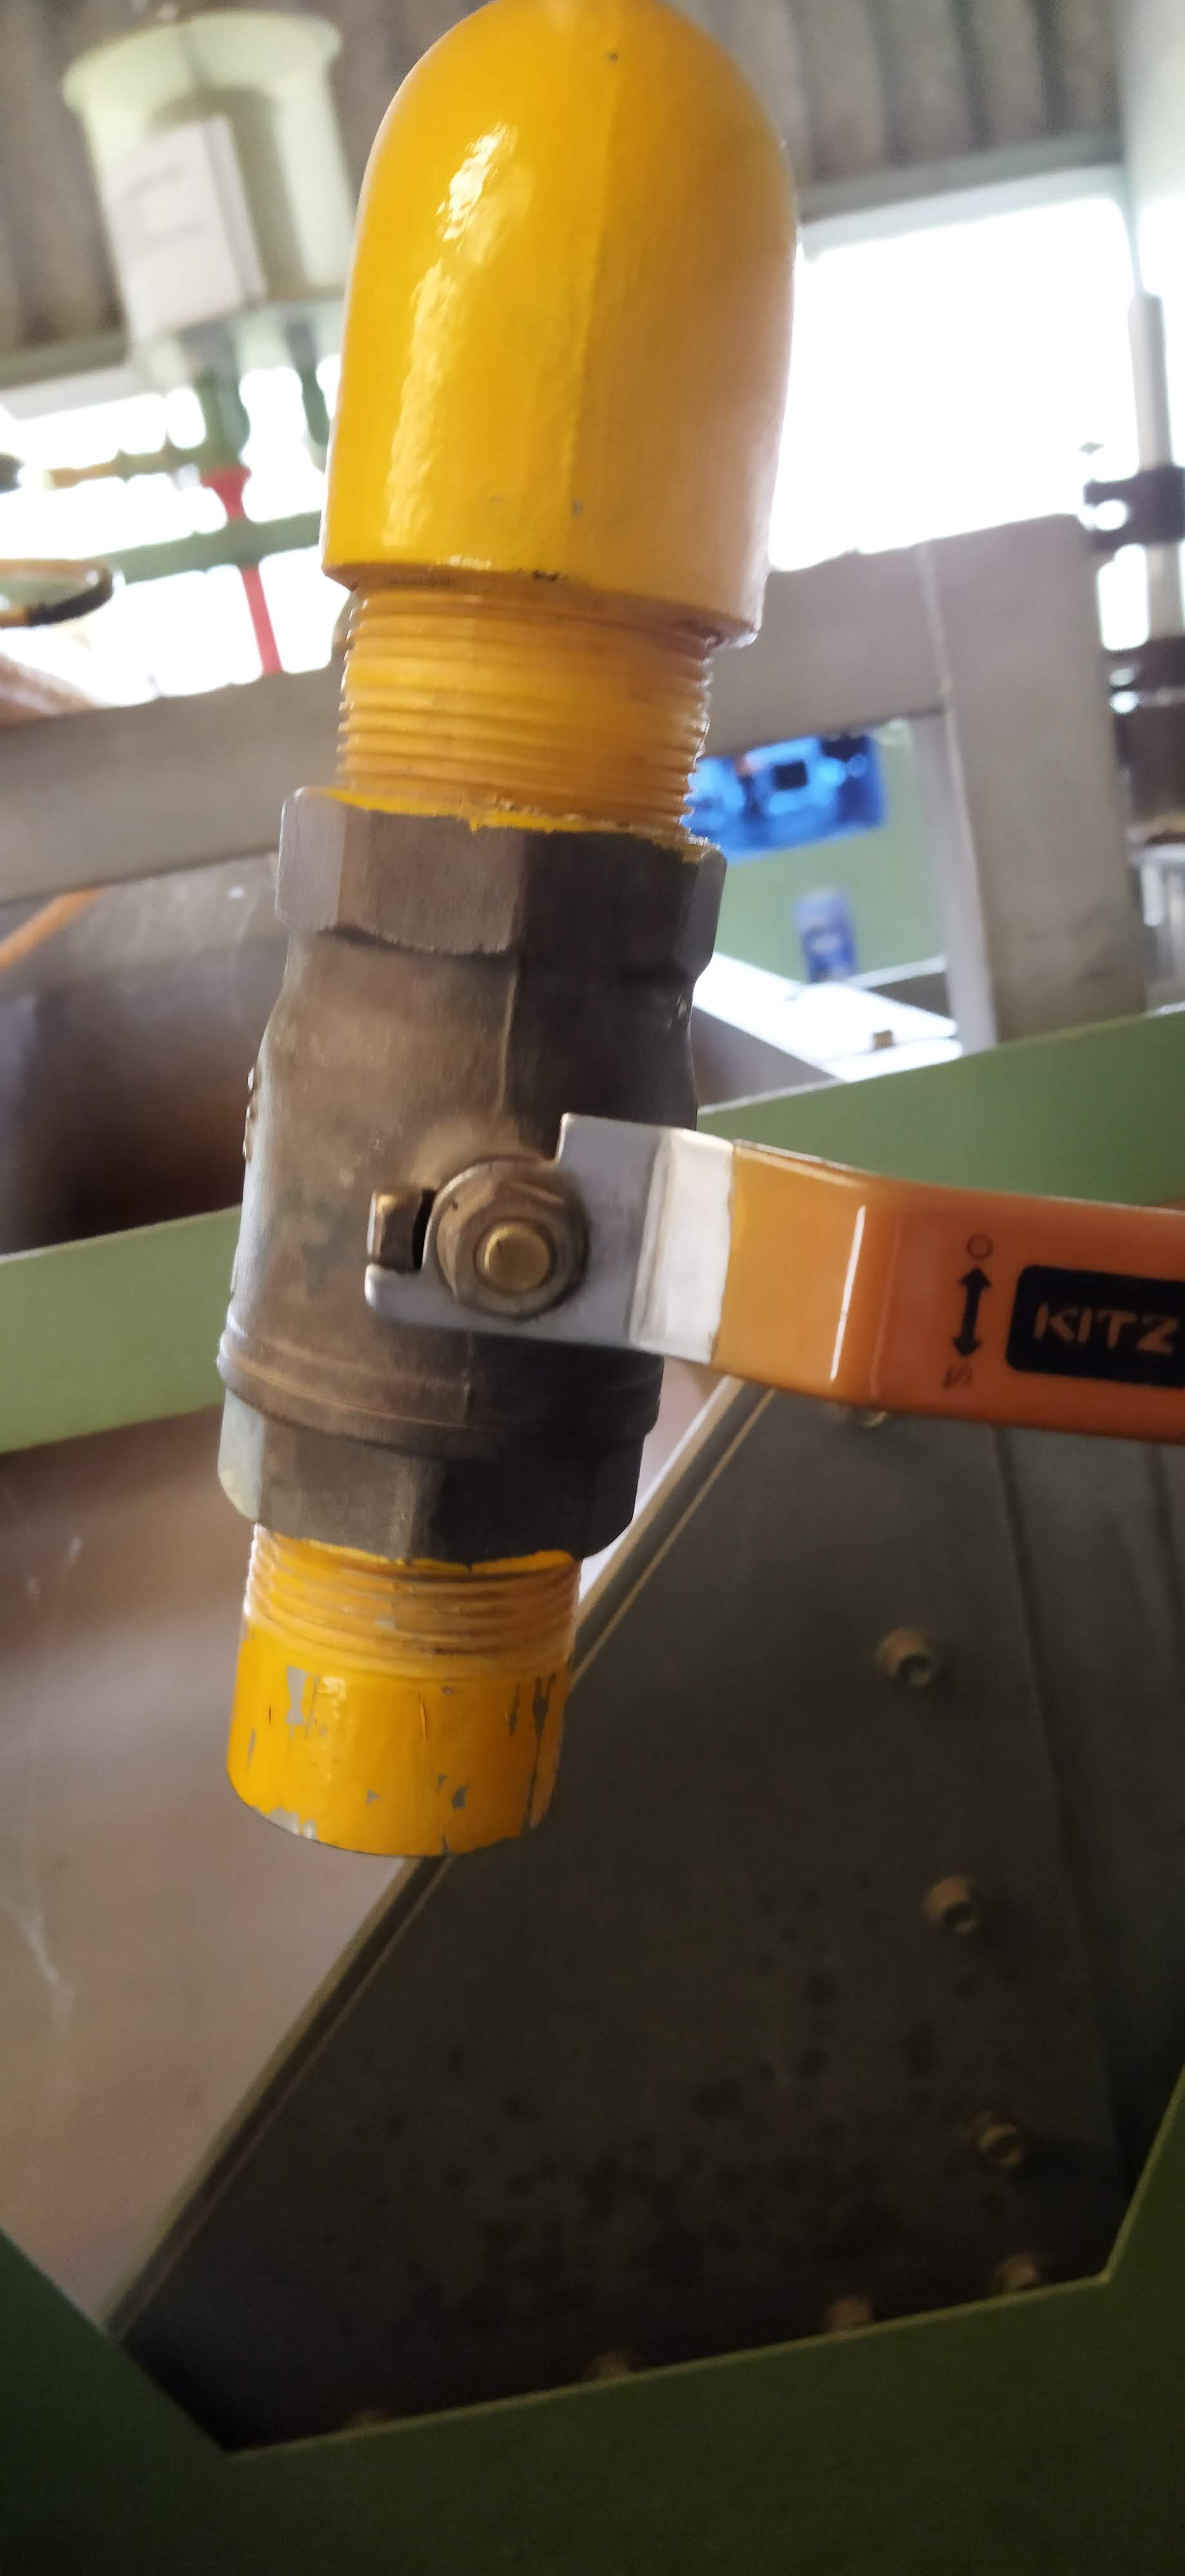
\includegraphics[width=\textwidth,height=0.3\textheight,keepaspectratio]{Figures/ballValve.jpg}
    \caption{Current discharge control unit}
    \label{fig:current_discharge_control_unit}
\end{figure}
\par
The valve is opened in steps by hand using the lever.
\par
Automation of this unit utilizes the existing ball valve. In addition, the opening and closing of the valve is automated using a motorized system that can open the valve in precise steps. To achieve the precise steps, the following consideration were made. 
\subsubsection{Design Considerations}
\begin{enumerate}
    \item The torque required to open and close the ball valve.
    \item The steps size or the number of steps the system can open the valve.
\end{enumerate}
\par
Based on these two considerations, the following two options were feasible.
\begin{enumerate}
    \item \textbf{Stepper Motor}\\
    This motor operates by accurately synchronizing position with the pulse signal output from the controller to the driver, achieving highly accurate positioning and speed control. Stepper motors feature high torque and low vibration at low speeds ideally below 1500rpm, ideal for applications requiring quick fixed positioning in a short distance \cite{wargula2017investigations}. Furthermore, stepper motor rotates with a fixed step angle typically 1.8 degrees for a 2-phase. However, to achieve this requires the use of a micro-step driver.
    \par
    Besides having full control of rotation and speed, the simple structure of stepper motors is achieved without using electrical components, such as an encoder within the motor. For this reason, stepper motors are very robust and have high reliability with very few failures. As for stopping accuracy, ±0.05° (without cumulative pitch errors) is very accurate\cite{wargula2017investigations}. Because the positioning of stepper motors is performed by open-loop control, and operated by the magnetized stator and magnetic rotor with small teeth, stepper motors have a higher follow-up mechanism toward commands than the servo motors. Also, no hunting occurs when stopping stepper motors.
    \item \textbf{Servo Motor}\\
    Servo motors run significantly faster than stepper motors, with speeds greater than 1500rpm \cite{halicioglu2016mechanisms}. This enables servo motors to be used with gearboxes to deliver much higher torque at useful speeds. They also deliver more consistent torque across the speed range of the motor. Unlike stepper motors, they do not have holding torque. Closed-loop operation enables the controller/drive to command that the load remain at a specific position, however, and the motor will make continual adjustments to hold it there. Thus, servo motors can deliver de facto holding torque\cite{halicioglu2016mechanisms}. The Servo motor rotates with a fixed step angle as low as 1 degree with or without the use of a driver. Furthermore, when powered, servo motors tend to move their shaft position to the zero position, a phenomenon referred to as hunting.
\end{enumerate}
\subsubsection{Motor Sizing and Selection}
\par
The motor shaft is required to turn $90^{0}$ in this application since the ball valve should only turn an angle of $90^{0}$ to open and return through the same angle to close. Accurate position control is therefore a key factor in the determination of the motor.
\par
The load torque that is acting on the motor is given by equation \ref{eq:2}
\begin{equation}
T=  F * r
\label{eq:2}
\end{equation}
\par
T is the torque required to overcome the ball valve and interface load, F is the maximum axial force on the motor(in this case it is the weight of both the ball valve and the interface) and r is the perpendicular distance from the point of action of force. The torque required to overcome ball valve and interface load was then calculated to be  approximately 5N/cm.

\subsubsection{Choice}
\par
Servo motor(MG996/12kg.cm/0.13s per 60 degrees turn) was selected for this operation. Its torque supply of 3kg/cm is above the required to overcome the load torque of both the ball valve and the interface. Furthermore, servo motor was selected to drive this unit because of the small step angle (1 degree) that it can turn as compared to a stepper with a typical step angle of 1.8 degrees. The smaller the angle, the more the number of steps hence the experiment could be conducted as many times as possible for higher accuracy. Furthermore, the fact that servo motors do not necessarily need a micro-step driver for their operation reduces the overall cost.

\subsubsection{Flow control sub-unit designs}
In order to support a stepper motor in place above the valve so that it can operate in place of the lever, the design had the following components:
\begin{enumerate}
    \item Motor cage\\
    This  unit is used to bolt down the motor to a rotating plate as shown in figure \ref{fig:holder1}
    \begin{figure}[p]
    \centering
    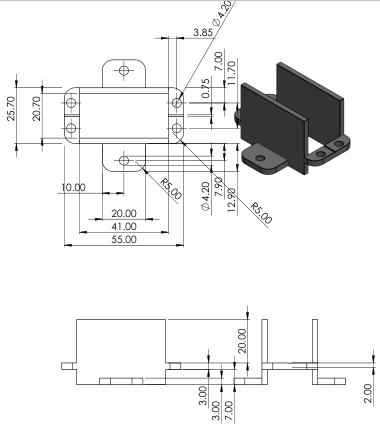
\includegraphics[width=0.6\textwidth]{Figures/servoMotorHolder.png}
    \caption{Servo Motor Holder}
    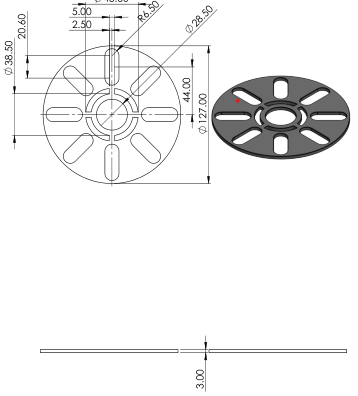
\includegraphics[width=0.6\textwidth]{Figures/servoMotorRotaryMount.png}
    \caption{Servo Motor Holder Mount }
    \label{fig:holder1}
    \end{figure}
    The design of the cage was guided by the dimensions of a standard servo motor(MG996 Metal Gear high Torque) which was 53.70mm by 19.70mm by 38.70mm.Taking into considerations the tolerance to allow for cooling of the motor during operation  and at the same time providing a firm support to the motor, the dimensions of the motor cage will be  55.00mm by 20.70mm by 20.00mm.
    \item Motor rotary mount\\
    This unit provides a base to bolt the motor cage as shown in figure \ref{fig:holder1}. It motor rotary mount will be supported by the supporting rods hinged to the valve with the help of serrated straps. The diameter of the mount was based on how far apart the the supporting rods were. Based on this, the diameter of mount will be 127.00mm.
    \item Interface \\
    The interface is used in place of the lever. It connects the rotor of the stator motor to the axle of the ball valve. Its design is as shown in the figure \ref{fig:motor_interface_n_rods}
    \item Supporting rods\\
    These rods supports the mounting base of the motor just above the ball valve. It is bolted to the discharge pipe through the two straps. Its design is as shown in figure \ref{fig:motor_interface_n_rods}
    \begin{figure}[p]
        \centering
        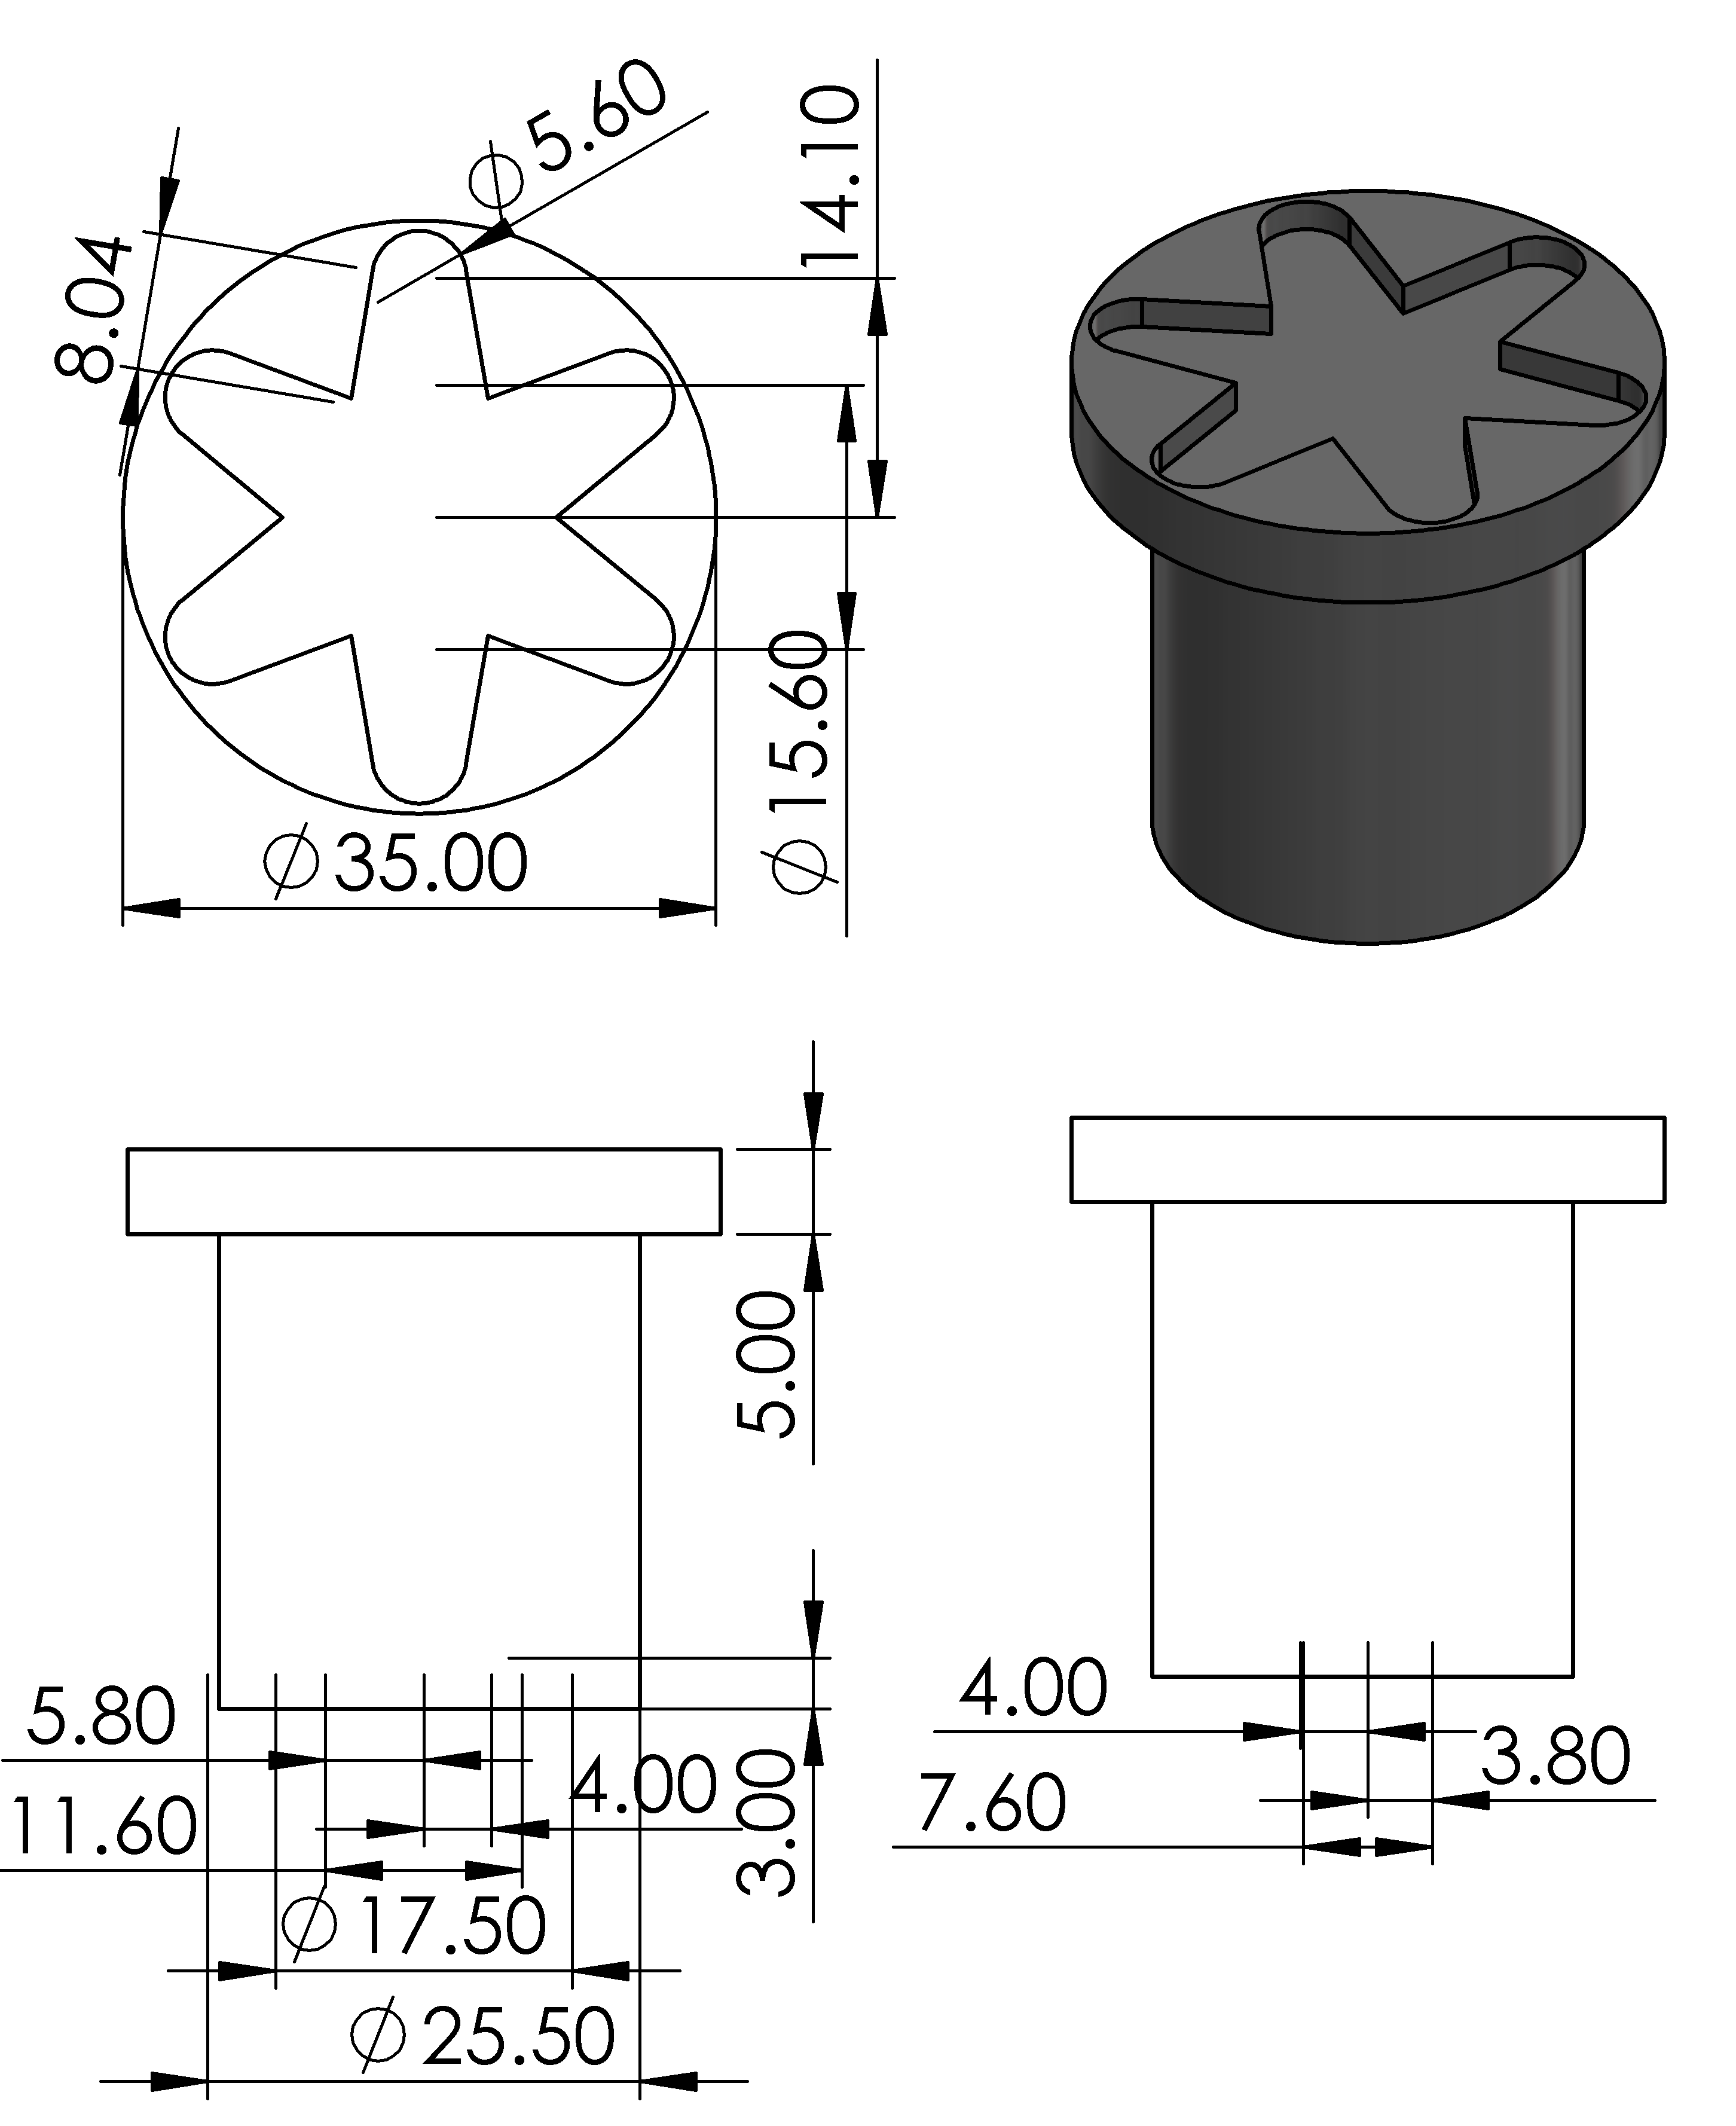
\includegraphics[width=0.6\textwidth, height=0.5\textheight]{Figures/interface.png}
        \caption{Motor-Valve interface}
        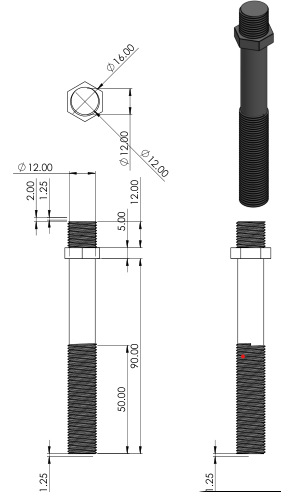
\includegraphics[width=0.6\textwidth, height=0.5\textheight]{Figures/supportingRods.png}
        \caption{Supporting rods}
        \label{fig:motor_interface_n_rods}
    \end{figure}
    \item Seratted Straps\\
    These are used to mount the whole unit on the circular surface of the pipe. Their design is as shown in the figure \ref{fig:motor_interface_n_rods}. Since the traps are hinged onto the ball valve casing, the design dimensions was guided by the diameter of the ball valve. The choice to use the serrated  valve was to enhance on the grip to the valve to avoid slidding.
    \begin{figure}[p]
        \centering
        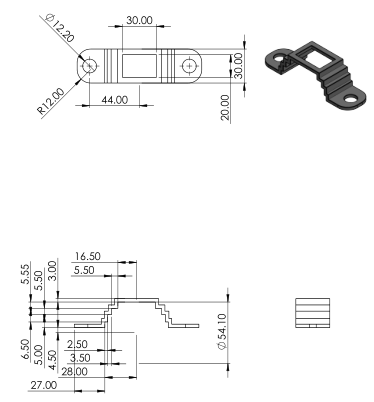
\includegraphics[width=0.8\textwidth, height=0.5\textheight]{Figures/s1.png}
        \caption{Top serrated strap}
        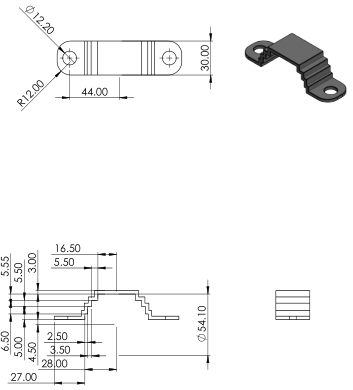
\includegraphics[width=0.8\textwidth,height=0.5\textheight]{Figures/ss33.PNG}
        \caption{Bottom serrated strap}
        \label{fig:top_n_bottom_straps}
    \end{figure}
\end{enumerate}
\par
 
\subsubsection{Flow diversion sub-unit}
\par
The sub-unit is responsible for diverting the discharge from the main pipe system to either the collection tank or into the main reservoir.
\subsubsection{Design Consideration}
The sub-unit is to have a faster response and large linear displacement capabilities Piezoelectric actuators and electromagnets were considered for this application.
\subsubsection{Piezoelectric Actuators}
Piezoelectric actuators are transducers that convert electrical energy into a mechanical displacement or stress based on a piezoelectric effect, or vice versa. They are used widely as a high precision positioning mechanism since they can control a small mechanical displacement at high speed, with the advantages of large generated force, stable displacement, and ease of use\cite{gao2020piezoelectric}. However, problems include insufficient displacement and the large voltage up to a few hundred volts, which is needed.
\subsubsection{Electromagnets}
Electromagnetic devices leverage the unique ability of magnetic metals such as iron to generate a magnetic field when electric current is applied. One of the biggest advantages offered by electromagnetic devices is durability. Unlike piezoelectric devices, which have the potential for shattered crystals, or electrostatic solutions with their required precise measurements, electromagnetic offerings can withstand high-volume, high-intensity use without suffering output or capacity loss\cite{yasumoto2018electromagnetic}. This makes them ideal for applications in which on-demand power and magnetism are required. Furthermore, as compared to piezoelectric actuators, electromagnets have a faster response and larger displacements which is actually ideal for our application.
\subsubsection{Choice}
JF-0530B DC12V push-pull electromagnet was selected as the main actuation mechanism for the flow diversion sub unit due to its faster response when energized as compared to piezoelectric actuators. Furthermore, as compared to electromagnets, piezoelectric actuators produce very small mechanical linear displacements as compared to electromagnets.
\clearpage
\subsubsection{Flow diversion sub-unit designs}
\begin{figure}[H]
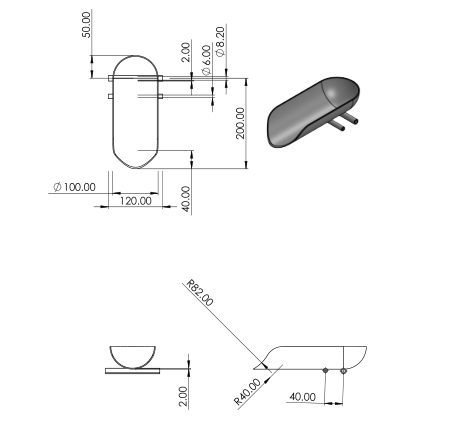
\includegraphics[width=0.9\linewidth]{Figures/flap.png}
\centering
\caption{Flap }
\label{fig:flap}
\end{figure}

\begin{figure}[H]
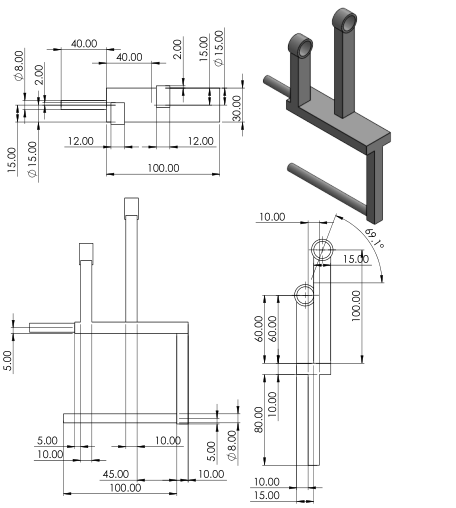
\includegraphics[width=0.7\linewidth]{Figures/ssholder.png}
\centering
\caption{Flow Diversion Support }
\label{fig:ssholder}
\end{figure}


\clearpage

\subsection{Discharge Collection Unit}
It is the core part of the experiment. The discharge collection unit comprises the flow diversion sub-unit, a discharge collection tank, an outlet valve, and weight and temperature measurements sub-units.
\subsubsection{Discharge collection tank}
The collection tank is used to temporarily collect the discharge from the pipeline during each phase of the experiment after which it is released to the main reservoir. Furthermore, it is the point at which both the weight and temperature of the discharge are measured. The discharge is to be collected for a specified amount of time after which it is released into the reservoir to allow for the next phase of the experiment. To ensure that there is motivated discharge into the main reservoir, the shape of the tank was critical hence the following design considerations were taken into account.
\subsubsection{Design Considerations}
\subsubsection{The Shape of the Tank}
\par
The shape of the tank not only influences how fast the discharge is released into the main reservoir but also the positioning of the outlet valve. Besides, it has an influence on the final weight of the discharge. This is so since a tank that holds discharge even after being released into the reservoir introduces a positive error into the load cells, which upon accumulation will eventually lead to incorrect results.
\begin{enumerate}
    \item Horizontal Cylindrical Tanks\\
    Horizontal cylindrical tanks provide the fastest way to release the discharge through a solenoid valve into the reservoir due to their shape. Additionally, there shapes ensures that no discharge is left into the tank. 
    \item Rectangular Tanks\\
    Rectangular tanks offer the same storage capacity as to cylindrical tank. However, unlike cylindrical tanks, these tanks may allow for accumulation of discharge which will affect the overall weight.
\end{enumerate}
\begin{figure}[ht]
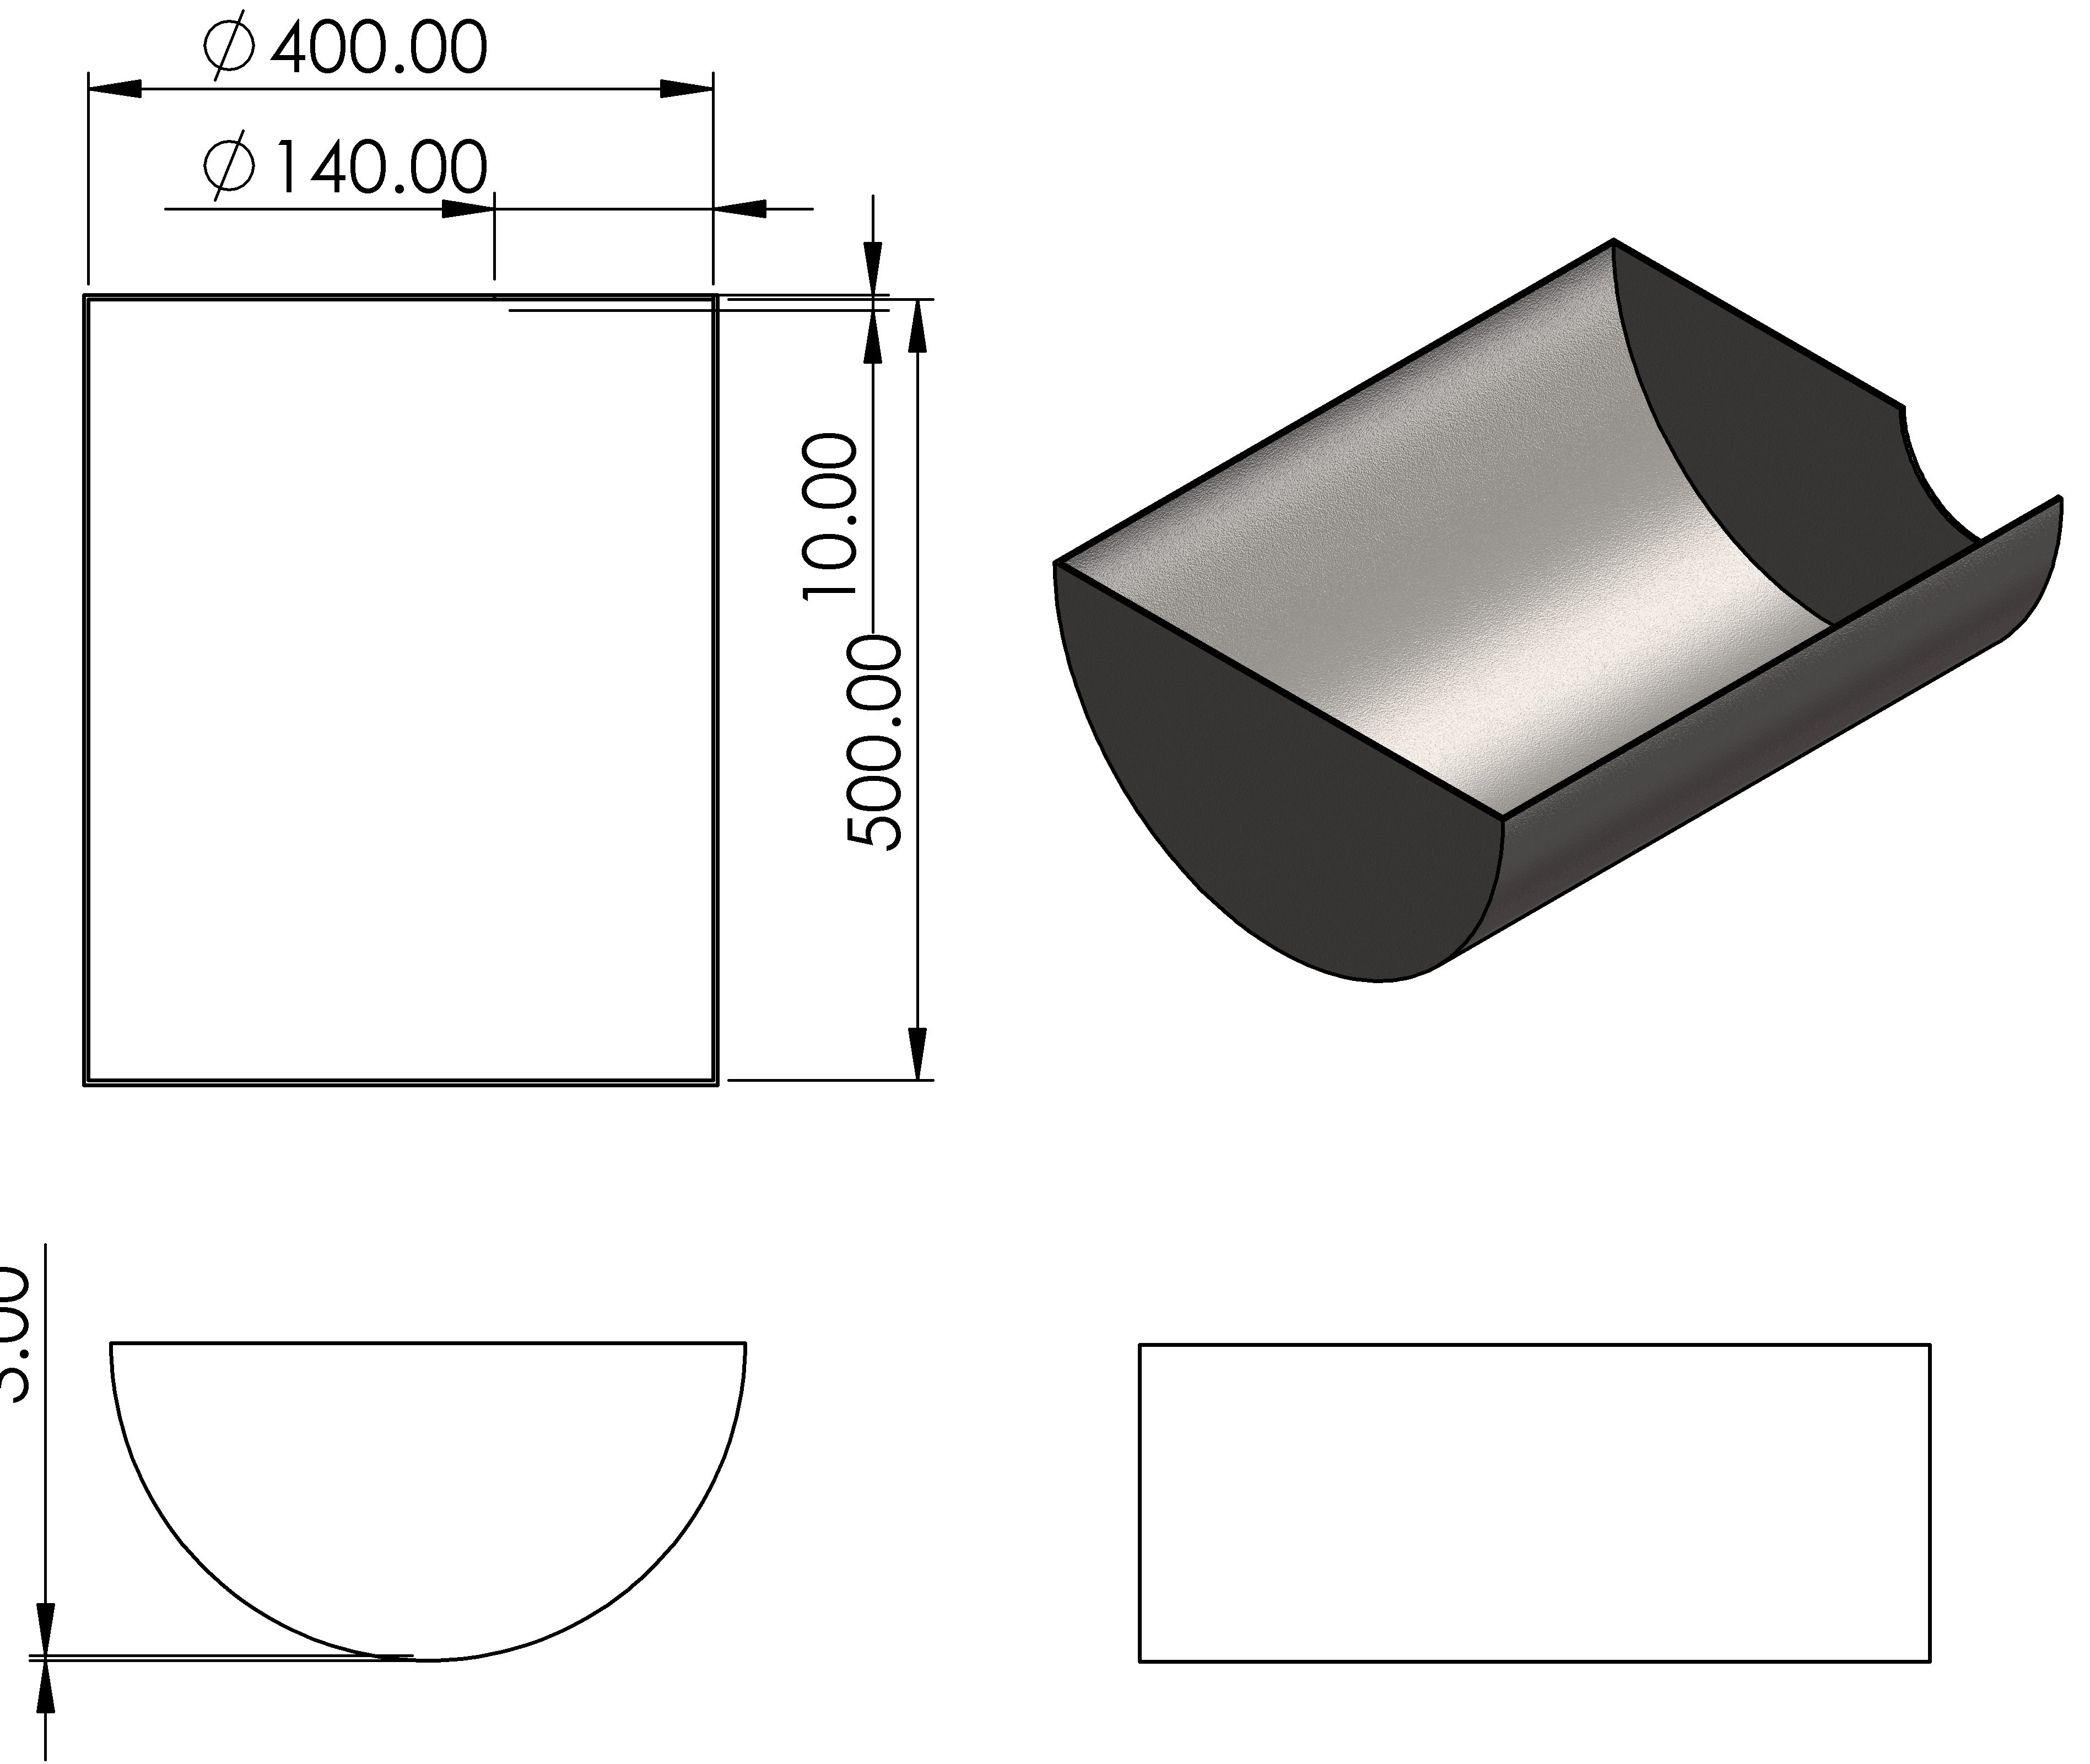
\includegraphics[width=0.9\linewidth]{Figures/tank.png}
\centering
\caption{Discharge Collection Tank }
\label{fig:tank}
\end{figure}

\begin{figure}[ht]
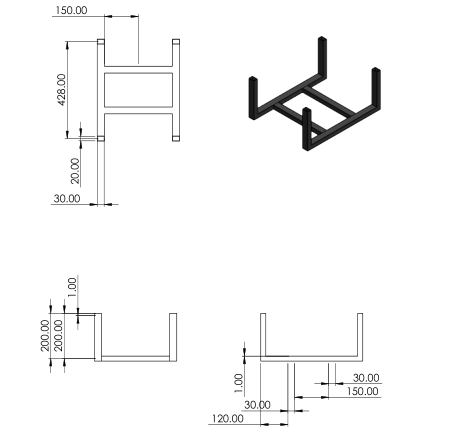
\includegraphics[width=0.9\linewidth]{Figures/Collection tank support.png}
\centering
\caption{Collection tank support }
\label{fig:Collection tank support}
\end{figure}

\subsubsection{Position}
\par
The positioning of the tank was also a critical aspect in the design. Ideally, the collection tank was to be either positioned directly just below the flow diversion unit or at the periphery of the main reservoir. Positioning the collection tank directly below the flow diversion unit mitigates the need for additional components like diverting pipes. This simply implies that the collection tank would just be provided with a holding mechanism for support upon which it is fitted with a solenoid outlet valve directly into the reservoir. On the contrary, positioning the collection tank at the periphery introduces the need for extra components. This includes a pump system to pump the discharge back into the reservoir which adds to the overall cost of the project. Positioning the collection tank below the diversion unit was the feasible option.
\par


\subsubsection{Choice}
\par
The horizontal cylindrical tank is ideal this application since as compared to the rectangular one, there is motivated discharge. This actually means that there is ease of flow of the discharge into he reservoir. Besides, with horizontal cylindrical tank, chances of discharge remaining into the tank are very minimal due to point concentration. This implies that errors in weight measurement due to discharge accumulation is minimized.
This sub-unit will be used to measure the weight of the discharge in the collection tank. The following approaches will be considered for this unit :

\begin{enumerate}
    \item Ultrasonic \newline
    Ultrasonic waves are used to determine the depth of the discharge in the tank. This is used together with the cross-sectional area of the tank, and the density of the discharge to determine the weight of the discharge based on the following equation \ref{eq:2}.
    Assuming a cylindrical collection tank, then mass is given by;
    \begin{equation}
     m= \rho*r^2 (h- h_1 )
    \label{eq:2}
    \end{equation}
    Where m is the mass of the collected discharge\newline $$\rho$$ is the density of the discharge\newline
    h is the height of the cylindrical tank \newline 
    $h_1$ is the height measured by the ultrasonic sensor.
    
    Considering the reliability and resolution of the ultrasonic waves, the resolution depends on the pulse rate of the ultrasonic wave generator. Furthermore, the use of ultrasonic waves requires the consideration of other factors such as the cross-sectional area and the shape of the tank. This will not be the case with the load cells.

    \item Load cells \newline
    A load cell is essentially a force transducer or force sensor. It is used principally to measure weight. Load cells are used for quick and precise measurements. Compared with other sensors, load cells are relatively more affordable and have a longer life span.
    The choice of the weight measurement unit was to use four load cells which are positioned just below the collection tank on the four edges of the tank holder. It should be noted that the collection tank and the tank holder introduce a positive error in the weight measurement hence the total weight is accounted for by the software. 
\end{enumerate}


\subsection{Interface and Control Unit}
\subsubsection{Interface sub-unit}
This sub-unit provides a means of interaction between the system and the user. Ideally, the sub unit enables the user to input instructions and control the discharge collection process to ensure that the right results are obtained. The choice of this system depended on  the following factors
\begin{enumerate}
    \item Aesthetics \\
    This refers to the perception of the user while operating the interface. It dictates how the user feels.For the case of our machine, the interface should provide for ease of navigation through various components and in terms of inputting commands like the time and the number of steps.
    \item Ergonomics \\
    This refers to the impact of the interface on the user, and the ease of operation. It dictates the ease and the efficiency the user experience while operating it.
    \item Size. \\
    This is the size of the operable part interface. It affects  contributes to the two factors mentioned above. 
\end{enumerate}
Based on the above considerations, the following choices were feasible:
\begin{enumerate}
    \item LCD With keypad \\
    \begin{figure}
        \centering
        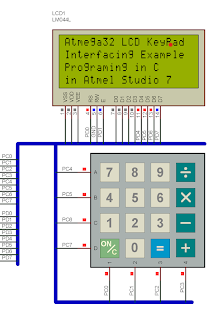
\includegraphics{Figures/controlInterface.png}
        \caption{LCD with keypad \cite{lcd_with_keypad}}
        \label{fig:lcd_with keypad}
    \end{figure}
    With this setup shown in figure \ref{fig:lcd_with keypad}, one can navigate, read and provide input where it is required on the LCD display using the keypad.
    \item LCD with touch \\
    One can navigate such interface easily by touching or using a virtual keyboard to provide input. This is shown in figure \ref{fig:lcd_with_touch}.
    \begin{figure}[!ht]
        \centering
        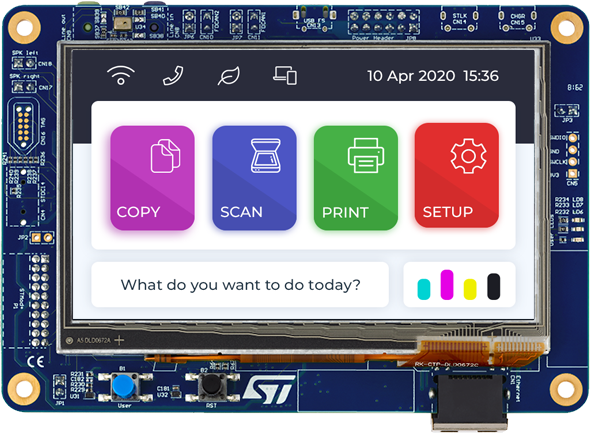
\includegraphics[width=0.6\linewidth]{Figures/lcdWithTouch.png}
        \caption{LCD with touch  \cite{lcd_with_touch}}
        \label{fig:lcd_with_touch}
    \end{figure}
    \\
     This kind of LCD communicates with the micro-controller through an 8-bit parallel interface. In order to support to touch, this LCD requires at least four ports(32 pins). 
    \item LCD with Knobs \\
    The interface can be controlled by a knob. Navigation from page to page, or from field to field is achieved by turning the knob. This is shown in figure \ref{fig:lcd_with_knobs}.
    \begin{figure}[!ht]
        \centering
        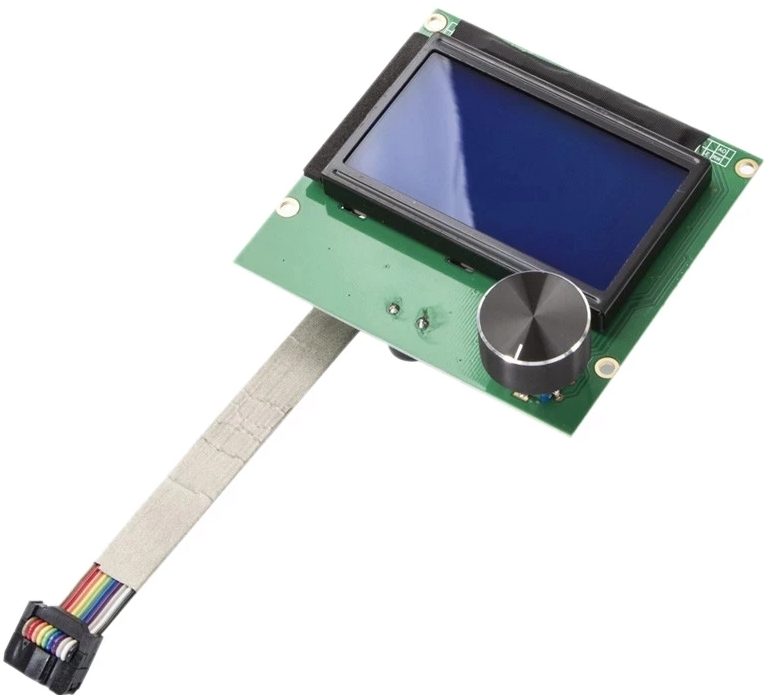
\includegraphics[width=0.6\linewidth]{Figures/lcdwithknob.png}
        \caption{LCD with knob \cite{noauthor_prusa_nodate}}
        \label{fig:lcd_with_knobs}
    \end{figure}
\end{enumerate}
\subsubsection{Choice}

 The optimum choice was to use of an LCD with touch capability. This choice serves all the requirements of an interface for this system. In addition, one can also improve on the design by just tweaking the GUI software with no hardware changes.

\clearpage
\subsubsection{Interface GUI design}
The design of the user interface is as shown in figure \ref{fig:GUI_interface}.
\begin{figure}[!ht]
    \centering
    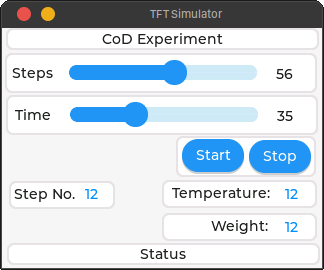
\includegraphics{Figures/interfacedesign.png}
    \caption{GUI interface}
    \label{fig:GUI_interface}
\end{figure}

\begin{figure}
    \centering
    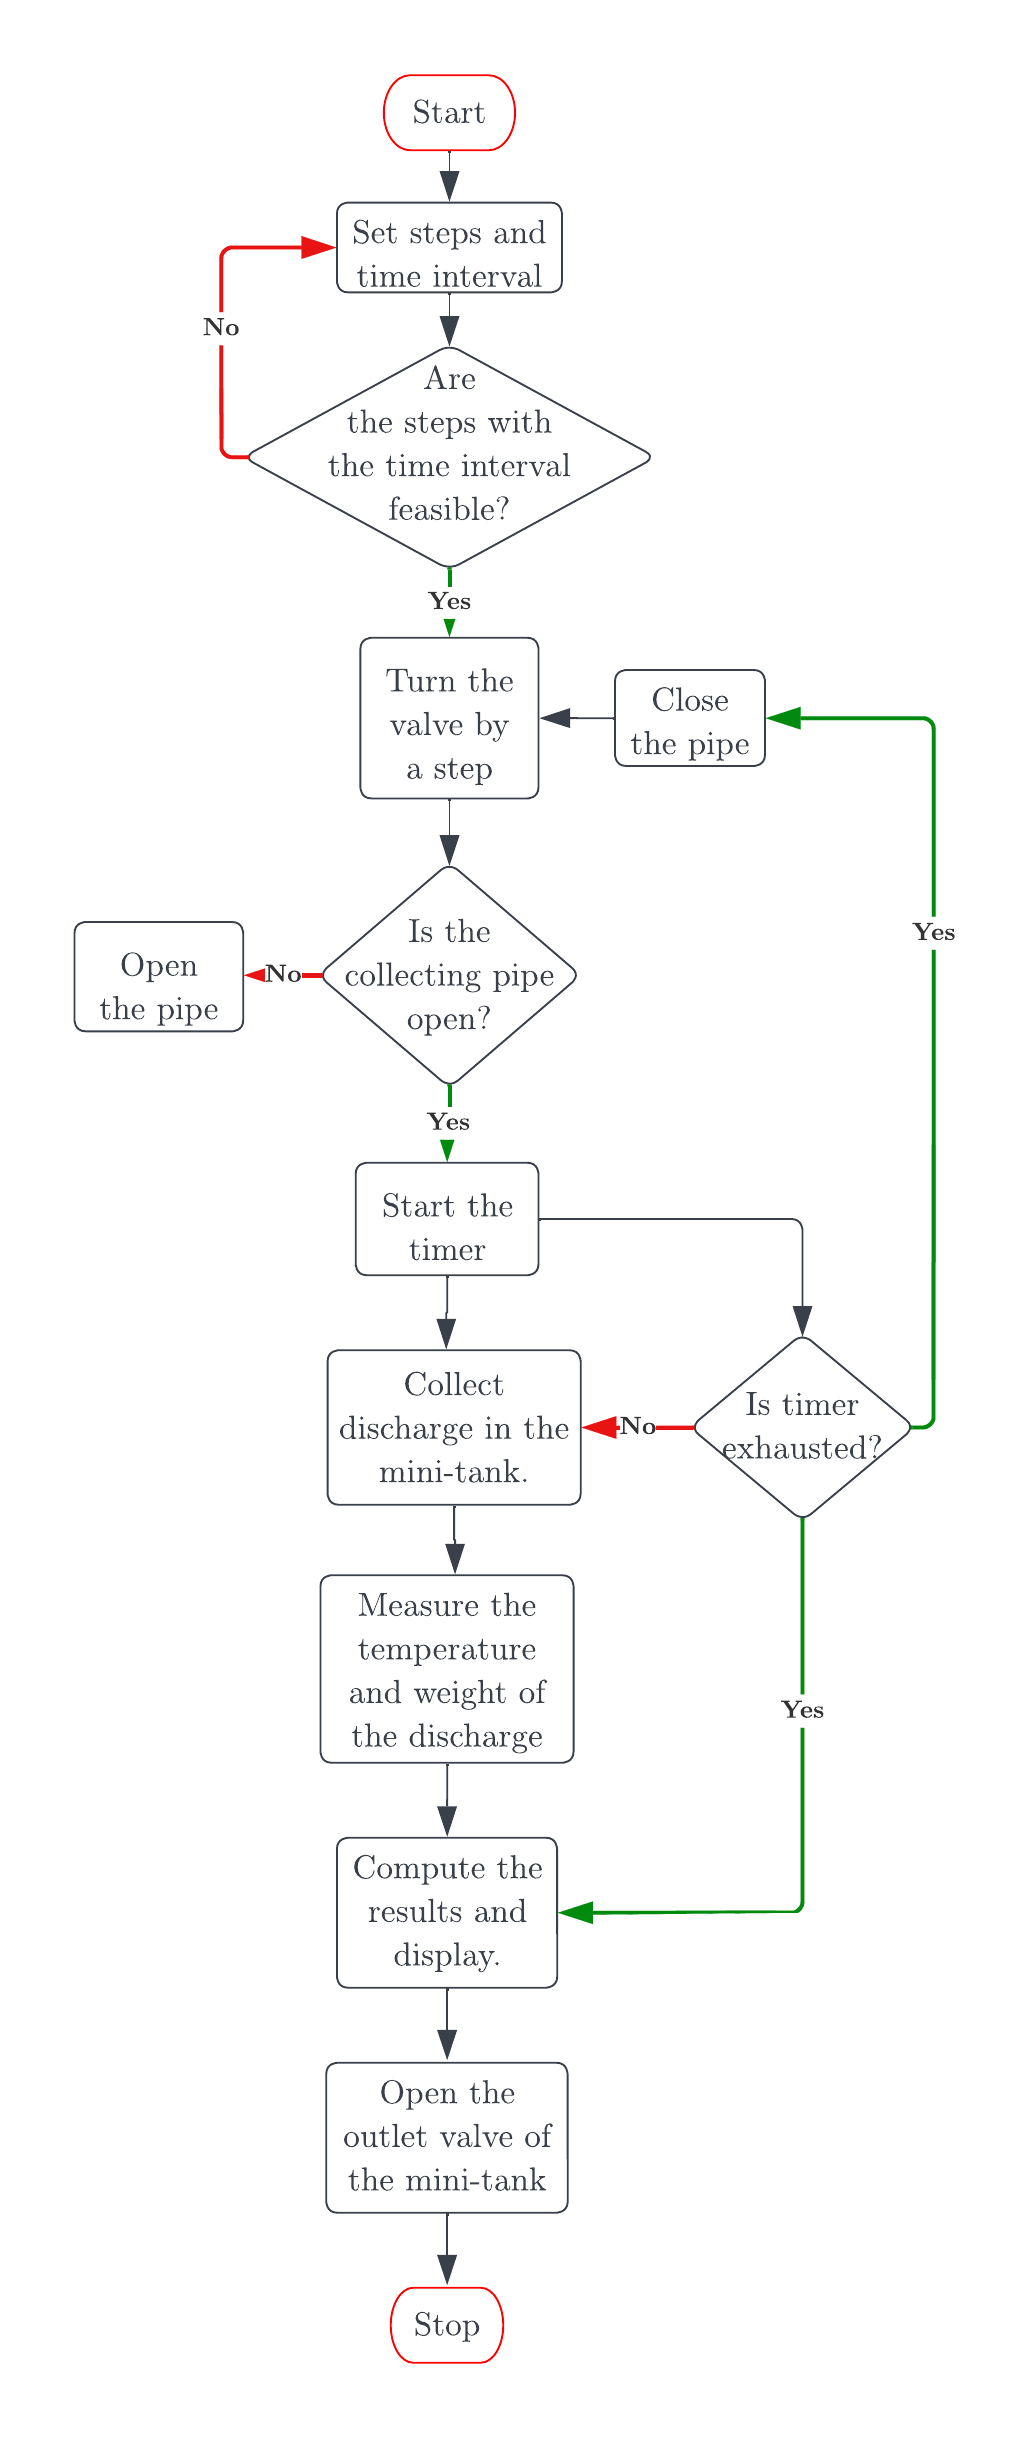
\includegraphics[width=\textwidth,height=\textheight,keepaspectratio]{Figures/Control_flow.png}
    \caption{Application logic}
    \label{fig:control_flow}
\end{figure}

\subsubsection{Processing and control sub-unit}
This sub-unit executes the application logic, send instructions to the actuators, and reads inputs from sensors in the system. It is responsible for synchronizing the GUI with the processes in the hardware. The unit monitors and controls the parameters of the input devices and generates output signals to implement desired tasks.
\par
As shown in figure \ref{fig:control_flow}, the user from the human interface will be prompted to start the experiment and input the number of steps and the time to conduct the experiment.The system will then automatically check several parameters like whether the number of steps and time interval are feasible. The system will then start the timer, collect the timer and at the same time measure both the temperature and weight of the discharge collected. The averages values from the temperature sensors and load cells are computed and the results displayed on the LCD. A solenoid valve then opens to allow the discharge to flow into the reservoir.

\subsubsection{Microprocessor Control Unit selection process}
The choice of a micro-controller for the processing unit was guided by the selected human machine interface, which was an LCD with touch capabilities. Figure \ref{fig:mcu selection} shows the considerations in the Microprocessor Control Unit selection process.
\begin{figure}
    \centering
    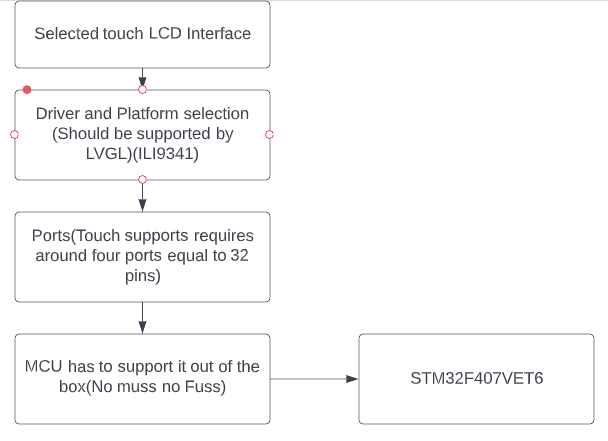
\includegraphics[width=0.9\linewidth]{Figures/mcu selection.png}
    \caption{Microprocessor Control Unit selection process}
    \label{fig:mcu selection}
\end{figure}

\begin{enumerate}
    \item Platform and Driver Support \\
    With an LCD with touch capabilities, the choice of the platform was between Light and Versatile Embedded Graphics Library (LVGL) and Mbed.The platform also had to support the driver used in the programming of the LCD. Based on the two platforms,LVGL was selected since it supports ILI9341, a driver intergrated circuit used in the control of LCDs. LVGL is an open-source graphics library providing everything you need to create embedded GUI with easy-to-use graphical elements, beautiful visual effects and low memory footprint.
    \item General Purpose Input Output(GPIO)s \\
    Touch support requires approximately four ports which is equivalent to thirty two pins. Finally, the MCU had to support it out of the box (No muss no fuss). The choice of the MCU was to accommodate for all the thirty pins.
    \item Processing Power \\
    This refers to the processing capacity of a micro-controller. A multi-core processor is faster and consumes more power as compared to a single-core processor. A multi-core processor can also render intense graphics on displays which would be essential for the LCD. The amount of input processing will guide one in choosing the best micro-controller or microprocessor for the task.
\end{enumerate}
Based on the above considerations, STM32F407VET6 was selected for the application.

